\chapter{Networks}

Today's lecture will focus on \emph{networks}. Networks are what let computers
communicate with each other. Computer network research permits communication
between computers across the internet, but there are more networks than just the
internet. Computers are networked together inside data centers, and such
computers can work together and solve tasks faster than normal computers can.
For example, many recent advances in AI have come from the increased computation
capabilities of using many networked computers.

We will review the following topics:
\begin{enumerate}
\item Types of networks (\S\ref{?})
\item Network Hardware (\S\ref{?})
\item Network Software (\S\ref{?})
\item Network Protections (\S\ref{?})
\end{enumerate}

%computer systems, a complex group of
%devices working together to perform a common task (or tasks). A user
%will interact with a computer through a variety of input and output
%devices (e.g. keyboards, mice, speakers, microphone, and monitors). A
%user's input will be processed, some computations will be performed,
%and then the resulting output will be displayed to the user. When most
%of us thinking about computers, we often think of a desktop or laptop
%computer, that come equipped with a keyboard, mouse, and monitor as
%seen in Figure~\ref{fig:hardware:computers};
%however, many things we interact with daily are computerized,
%including cell phones, cars, traffic lights, smart watches,
%televisions, and manufacturing lines. Today each of these items
%have sensors to perceive the real world, use an embedded computing
%device to understand the sensory input, and use a combination of
%display and mechanical devices to interact with the real world.
%
%\begin{example}
%For intersections across busy roadways, some traffic lights are
%computerized to optimize road traffic. These lights will stay
%green along the busier of the two roads, and use cameras or
%pressure sensors to detect the presence of cars along the less
%busy of the two roads, thus switching to allowing the cars on
%the less busy road to cross when it arrives. Overall, providing
%a less congested intersection by relying on an embedded computer.
%\end{example}
%
%Today we will introduce three fundamental parts of computer systems:
%input and output devices, memory, and the central processing unit (CPU).
%These components work together to perform the basic building blocks of
%input processing, storage, control, and output. Understanding how the
%three parts work together will allow us to create powerful information
%processing tools. We will introduce each of these parts in turn.
%In figure~\ref{fig:hardware:overview}, we see how these parts come
%together to form a computer system (similar to the ones you'll use
%to program in this course).
%
%\begin{figure}
%	\centering
%	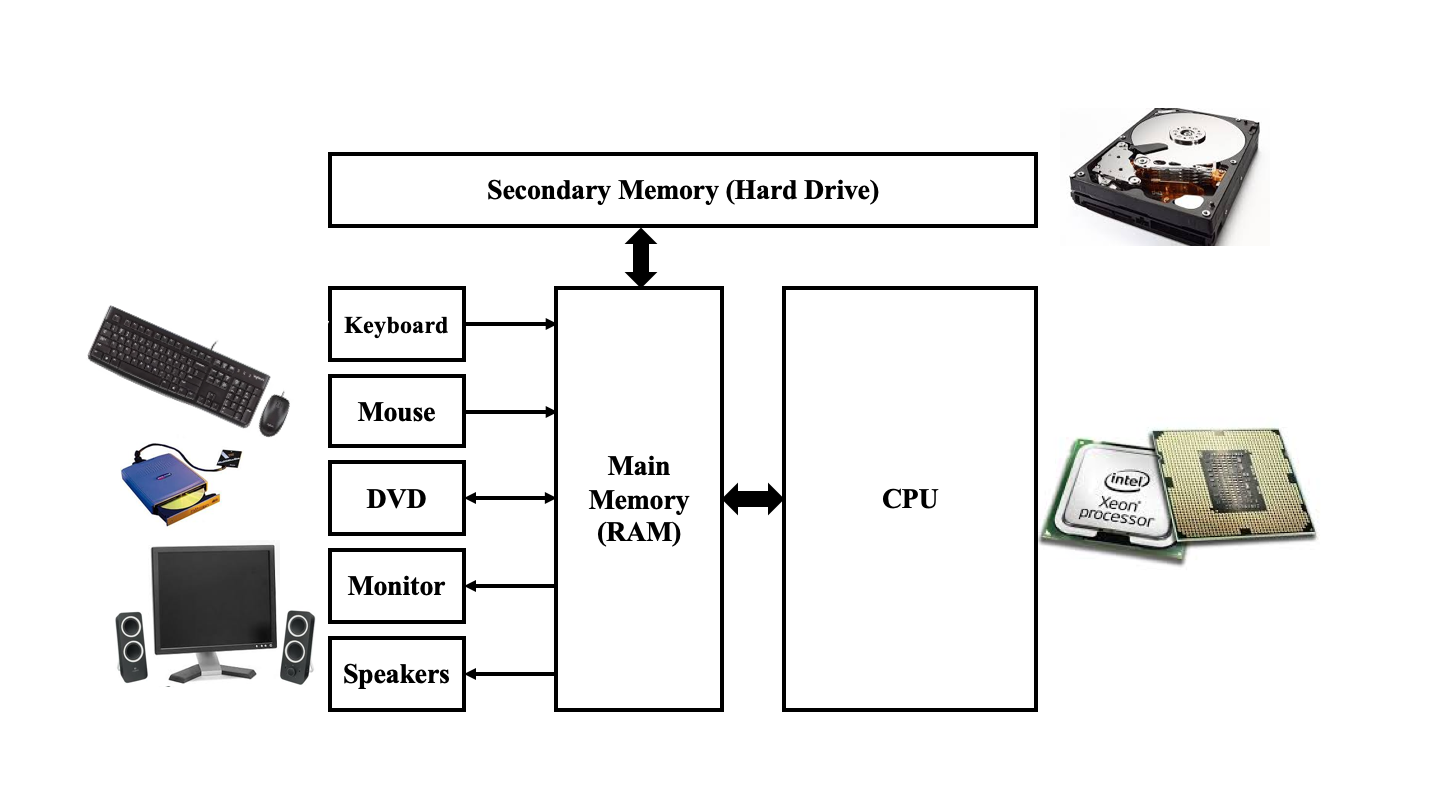
\includegraphics[width=0.85\textwidth]{images/cs_intro_hardware_overview.png}
%	\caption{Interconnected parts of a computer system (keyboard, mouse,
%                 monitor, DVD player / burner, speaker, hard drive, CPU).}
%	\label{fig:hardware:overview}
%\end{figure}
%
%\section{Input and Output Devices}
%
%We will begin by discussing input and output devices. These devices
%allow the computer to interact with users and the world directly. Without
%these devices, a computer system would be very boring, always performing
%the same computation each time it's used. Even if it did compute a different
%value we would be unable to examine the value. A computer needs to be
%able to accept input and allow output. The first computers would occupy
%a large room in an office building and connect to a terminal
%(a keyboard and a text screen) in another room for users to interact
%with. Thanks to Moore's Law, computers many orders of magnituted more
%powerful can fit in the palm of your hand. Likewise, the variety of input
%and output devices has multipled. We still have the keyboard and monitor,
%we've added the mouse for interacting with graphical displays. Today's
%phones are more computer than phone, coming equipped with: speakers,
%microphones, touch screens, cameras, fingerprint scanners, radio transmitters,
%and much more. Computers even come embedded in other devices like cars,
%traffic lights, X-ray machines, and thermostats to both control and
%monitor the devices. As shown in Figure~\ref{fig:hardware:overview},
%these devices connect to the rest of the computer through the computer's memory.
%This kind of input and output is called memory mapped I/O (input and output).
%Creaters of input (or output) devices are assigned a section of the
%computer's memory to write (read resp.) data. The computer will then read
%(write resp.) data to those locations to communicate with the given device.
%The creaters of these devices, agree upon a known format to read and write data.
%
%\begin{example}
%You can think of this communication between devices and computer similar to
%leaving messages for a friend in a locker. Only you and your friend have
%access to this locker, which only holds space for one message. The format
%you agree upon is which language you'll use to speak (e.g. English) and any
%special keywords or phrases. You might agree with your friend, that if either
%of you write a message saying ``The morning is upon us'' that the other will
%wait until ``The night has come'' before leaving any new messages.
%\end {example}
%
%The format that devices and computers communicate in are generally very simple
%and structured to permit fast and easily understandable communication for
%computers and devices.
%
%\begin{example}
%A monitor is a graphical display for computers. Let's consider a monitor
%connected to a computer that only displays in black and white images
%that are 20 x 20 pixels large. The monitor and keyboard agree upon using
%the following format to communicate. The format is black and white images
%that are 20 x 20 pixels large. Each pixel's value is represented at 0 for
%black and 1 for white. Then an image is represented as a 400 = (20 x 20) long
%sequence of pixel values. The sequence is ordered left to right, top to bottom.
%Now that both the monitor and computer agree upon the communication format, the
%computer can write images to the section of memory dedicated to the monitor
%and the monitor will read the image and display the image on it's screen.
%Figure~\ref{fig:hardware:monitor_image} displays an example image, a 
%20 x 20 chekerboard with its encoding.
%
%\emph{Note: while this is a simplified example, this is similar to how modern
%graphical displays communicate with computers}.
%\end{example}
%
%\begin{figure}
%	\centering
%        \hspace{0.5cm}
%	\begin{minipage}{0.45\textwidth}
%		
\includegraphics[width=0.90\textwidth]{images/checkered_image.jpg}
%	\end{minipage}
%        \begin{minipage}{0.45\textwidth}
%		\scriptsize
%\begin{verbatim}
%0 1 0 1 0 1 0 1 0 1 0 1 0 1 0 1 0 1 0 1
%1 0 1 0 1 0 1 0 1 0 1 0 1 0 1 0 1 0 1 0
%0 1 0 1 0 1 0 1 0 1 0 1 0 1 0 1 0 1 0 1
%1 0 1 0 1 0 1 0 1 0 1 0 1 0 1 0 1 0 1 0
%0 1 0 1 0 1 0 1 0 1 0 1 0 1 0 1 0 1 0 1
%1 0 1 0 1 0 1 0 1 0 1 0 1 0 1 0 1 0 1 0
%0 1 0 1 0 1 0 1 0 1 0 1 0 1 0 1 0 1 0 1
%1 0 1 0 1 0 1 0 1 0 1 0 1 0 1 0 1 0 1 0
%0 1 0 1 0 1 0 1 0 1 0 1 0 1 0 1 0 1 0 1
%1 0 1 0 1 0 1 0 1 0 1 0 1 0 1 0 1 0 1 0
%0 1 0 1 0 1 0 1 0 1 0 1 0 1 0 1 0 1 0 1
%1 0 1 0 1 0 1 0 1 0 1 0 1 0 1 0 1 0 1 0
%0 1 0 1 0 1 0 1 0 1 0 1 0 1 0 1 0 1 0 1
%1 0 1 0 1 0 1 0 1 0 1 0 1 0 1 0 1 0 1 0
%0 1 0 1 0 1 0 1 0 1 0 1 0 1 0 1 0 1 0 1
%1 0 1 0 1 0 1 0 1 0 1 0 1 0 1 0 1 0 1 0
%0 1 0 1 0 1 0 1 0 1 0 1 0 1 0 1 0 1 0 1
%1 0 1 0 1 0 1 0 1 0 1 0 1 0 1 0 1 0 1 0
%0 1 0 1 0 1 0 1 0 1 0 1 0 1 0 1 0 1 0 1
%1 0 1 0 1 0 1 0 1 0 1 0 1 0 1 0 1 0 1 0
%\end{verbatim}
%        \end{minipage}
%	\caption{An example checkered image and its encoding --- newlines and spaces added for readability.}
%	\label{fig:hardware:monitor_image}
%\end{figure}
%
%\section{Memory}
%
%Another fundamental part of a computer, is the memory. By memory, we mean the
%ability to store and recall data. This is very similar to physical storage of
%items. Figure~\ref{fig:hardware:storage} shows three storage locations ---
%a storage closet, a garage, and a warehouse. Each of the three locations
%have tradeoff between convenience of location and storage capacity. The
%closet can contain a few things and is the same room you need it. The garage
%can fit even more things and is only a walk outside (or through) your home,
%and the warehouse can fit practically anything you would want to store but you
%have to drive to the warehouse to pick-up or store your items.
%Similarly, a computer's memory makes the same trade-offs.
%
%There are two major types
%of memory, Main Memory (RAM), and Secondary Memory (e.g. hard disks, solid-state
%drves, tape drives, etc.) Main memory is volatile, meaning that the contents
%of the memory is not preserved when a computer is turned off and back on. On the
%other hand Secondary Memory, is meant to be persistent (the opposite of volatile).
%Main Memory can be thought of as the ``scratch paper'' the computer uses for
%computations. Computers will also use Main Memory as a conduit for communicating
%between the CPU and all other parts of the computer. Staying with the analogy
%from Figure~\ref{fig:hardware:storage} main memory is closer to a garage
%(where you can lose items when you turn off the lights) --- there is enough
%room to fit most items you use regularly and is close enough to not worry
%about the time it takes to get to the garage.
%
%In most modern computers,
%programs are treated as data. That is the individual instructions that combine
%to form a program are stored in memory just as data is. It is the job of the
%computer to properly understand if a segment of memory is data or a program.
%The computer is able to fetch data from Secondary Memory to Main Memory or
%persist data in Main Memory to Secondary Memory when needed; however,
%this process of transferring data between Secondary and Main Memory can
%cost a lot of time relative to keeping data in Main Memory only.
%
%\begin{figure}
%	\centering
%	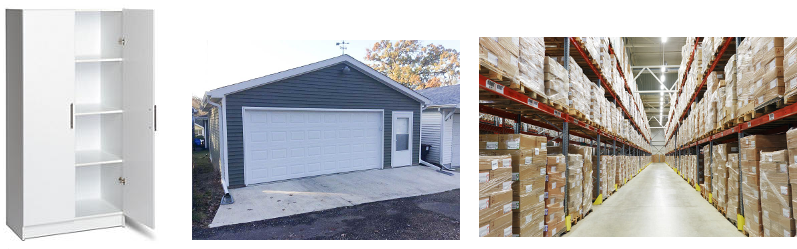
\includegraphics[width=0.85\textwidth]{images/storage.png}
%	\caption{Storage closet, garage, and warehouse trading off between
%                 capacity and locality.}
%	\label{fig:hardware:storage}
%\end{figure}
%
%\section {Central Processing Unit}
%
%The final part of a computer we will introduce today is the central processing
%unit (CPU) --- processor, main processor, etc. The CPU is the physical
%circuitry of a computer that performs instructions. The CPU has several key
%components: the control logic, arithmetic and logic unit (ALU), registers,
%program counter (PC), and clock. These components work together to 
%fetch, decode, and execute all instructions --- the building blocks of all programs.
%Instructions vary between different brands of CPUs, but, in general, they will
%include arithmetric, control, read (from memory), and write (to memory) functionalities.
%Example~\ref{ex:hardware:instr} shows several instructions
%that together would perform \ic{x = x + y}, given \ic{x} is stored in memory
%location 16 and \ic{y} at memory location 20. These instructions are quite low
%level, and harder for humans to read than the programs we will write in this course.
%However, the programs we write will be translated into these instructions to be
%easily understood and executed by the CPU.
%
%\begin{example}
%\label{ex:hardware:instr}
%\begin{verbatim}
%load R1 16    -- Load value at memory location 16 into register 1
%load R2 20    -- load value at memory location 20 into register 2
%add  R1 R2 R1 -- add the value in register 1 to the value in register 2
%                 and store in register 1
%store R1 16   -- store the value in register 1 to memory location 16
%\end{verbatim}
%\end{example}
%
%A key component of a CPU is its clock. The clock allows the CPU to progress in time,
%triggering the time to progress from time \ic{t} to time \ic{t + 1}. A single time
%segment is referred to a clock cycle. You might have heard about a computer's CPU
%speed (e.g. my computer runs at 2.4 GHz = 2.4 billion clock cycles a second). This
%is determined by how fast the clock transitions from one time to the next. This
%clock drives the progress of the CPU. The time an instruction takes is measured
%in instruction cycles. The rate of the CPU's clock is determined by the slowest
%operation of the CPU (e.g. fetch, decode, execute stage).
%
%In addition to clocks, the CPU contains a group of memory locations called registers.
%A single register is capable of holding a single word of information (the smallest
%unit of data in a computer). The key benefit of registers is the ability for the
%CPU to immediately read and write the contents of the CPU. The value of registers
%can be updated on each clock trigger (i.e. on the change from time \ic{t} to \ic{t + 1}).
%Most modern CPU's will have between 16 and 64 registers that programs may use.
%For comparison, accessing Main memory can take 10's or even 100's of instruction
%cycles to access while registers are immediately available to the CPU.
%
%The control unit and program counter (PC) will fetch, decode, and output the
%controls for the execution of each instruction. The program counter holds the
%location of the next instruction to be executed. The next instruction is then
%fetched to the CPU. The CPU's control unit then decodes the fetched instruction
%and outputs control signals (commands) to main memory and the ALU. The CPU may
%read data from memory (e.g. store) and then the ALU will then execute the action
%specified by the control unit (e.g. add, subtract, multiply, compare to 0, etc.),
%and then possibly write the output to memory.
%
%In most computers, the CPU and its constiuent parts are responsible for all
%computing needs of the computer. In some select systems, there will be additional
%hardware to perform specialized operations (e.g. graphics processing units for
%processing / producing images). It is the CPU's responsbility to control the
%computer and coordinate with devices to execute programs. As such, the CPU
%has seen a quick evolution to increase it's processing power. Electrical
%engineers, originally focused on making the CPU smaller and smaller and thus
%quicker, following Moore's Law : every two years the size of a CPU shrinks
%in half. Additionally, CPU's were designed with a pipelining architecture
%(i.e. multiple instructions are executed in quick succession). This is done
%by noting that each stage of the five stages --- fetch, load,  decode, execute,
%and store --- can be performed independently. Thus, while one instruction is
%being executed, the next instruction can be decoded. Figure~\ref{fig:hardware:pipeline}
%shows how pipelining is peformed by executing the different parts of the pipeline
%in parallel for five consecutive instructions.
%
%Due toe the decline of Moore's Law in recent years, many CPU designers focus on
%increasing processing power by improving parallelism (i.e. being able to execute
%multiple instructions at a time). This allows instructions that do not depend
%on each other to be executed at a time. These CPU are refered to as multi-core,
%as they have multiple cores that each have thier own set of registers, control unit,
%ALU, and PC but share main memory and a single clock. In this class we, will not
%teach how to effectively harness parallel programming, but note that this is
%an important progress in how hardware has evolved.
%
%\begin{figure}
%	\centering
%	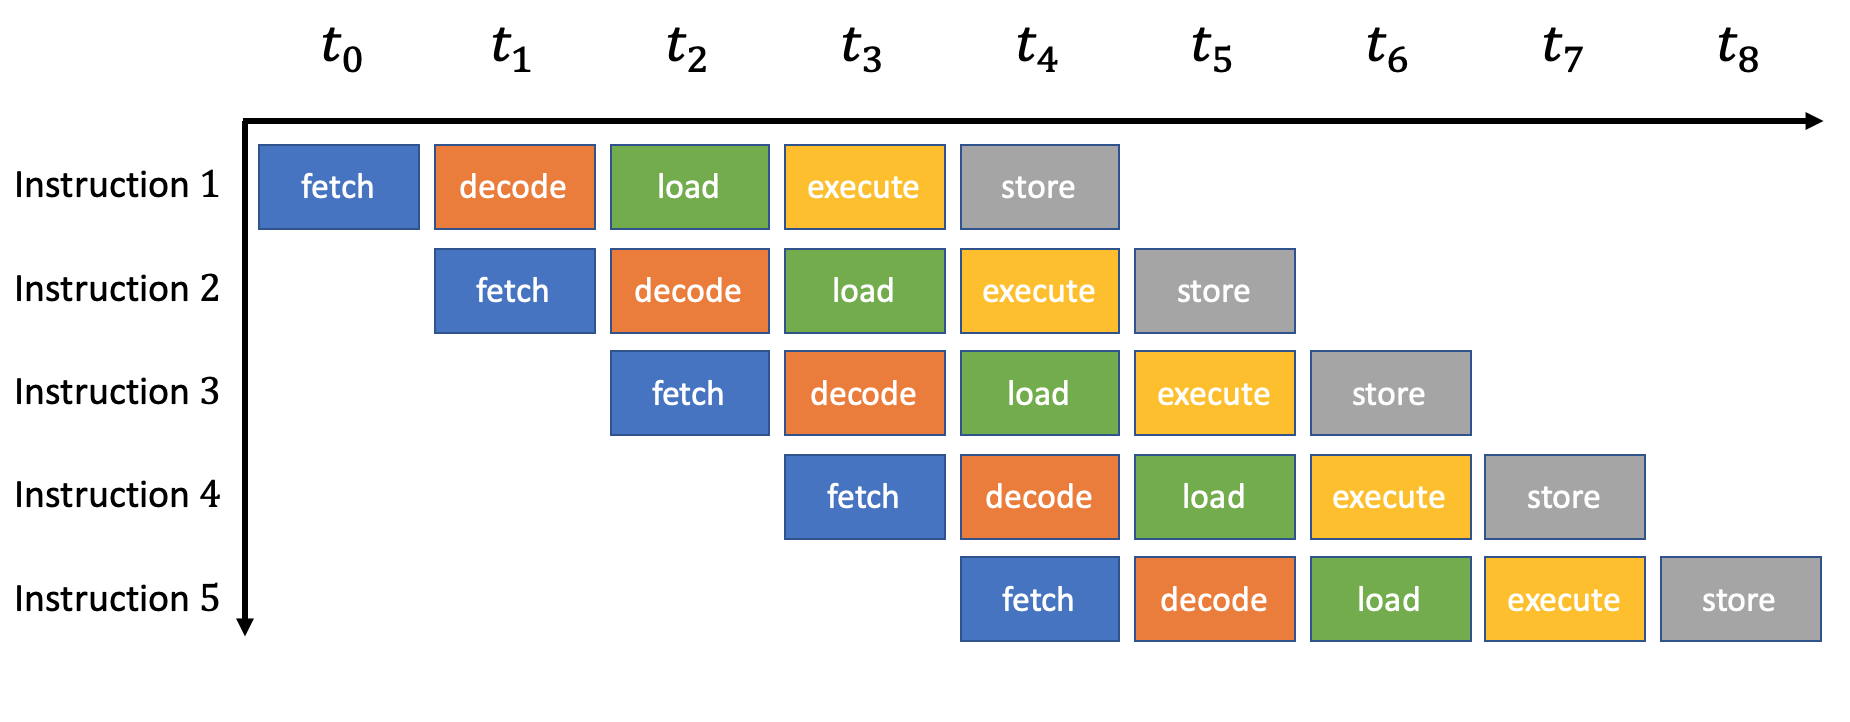
\includegraphics[width=0.85\textwidth]{images/pipeline.png}
%	\caption{Instruction Pipelining}
%	\label{fig:hardware:pipeline}
%\end{figure}
%
%
%
%\section {Conclusion}
%In this chapter, we covered the three fundamental parts of a computer system:
%input and output devices, Main and Secondary Memory, and the CPU. We discussed
%their roles, relationships, and basic capabilities. I hope that this will help
%you better understand how hardware works at a high level to better improve how
%to write programs that will eventually run on these computer system. In the
%next chapter we will begin discussing the concept of Software and how its
%similarities and differences to hardware and where the boundary between the two
%lies.
%
%\section {Learning Objectives}
%After covering this chapter, you should be able to answer the following questions:
%
%\begin{enumerate}
%\item What three parts comprise a computer system?
%\item What are examples of common input and output devices?
%\item Name an uncommon example of a computer system and explain how it may work.
%\item How does memory mapped input and output work?
%\item Name four kinds of memory devices and explain the difference between Main and Secondary Memory.
%\item What parts comprise the central processing unit (CPU)?
%\item Describe three possible methods to increase the computation power of a CPU.
%\end{enumerate}
